\documentclass{article}

% Language setting
% Replace `english' with e.g. `spanish' to change the document language
\usepackage[english,russian]{babel}
\usepackage{amsmath}

%графика
\usepackage{wrapfig}
\usepackage{graphicx}
\usepackage{pgfplots}
\usepackage{tikz}


\usepackage{tcolorbox}

% Set page size and margins
% Replace `letterpaper' with `a4paper' for UK/EU standard size
\usepackage[letterpaper,top=2cm,bottom=2cm,left=3cm,right=3cm,marginparwidth=1.75cm]{geometry}

% Useful packages
\usepackage{amsmath}
\usepackage{amssymb}
\usepackage{graphicx}
\usepackage{fixltx2e}
\usepackage[colorlinks=true, allcolors=blue]{hyperref}

\usepackage{geometry}
\geometry{left=25mm,right=25mm,
 top=25mm,bottom=25mm}

\title{Quantitative Analytics.\\
Lectures. Week 3-4. \\
Interest rates. Процентные ставки.}
\author{Kamenskaya Elizaveta}

% Колонтитулы
\usepackage{fancyhdr}
\pagestyle{fancy}
\renewcommand{\headrulewidth}{0.1mm}  
\renewcommand{\footrulewidth}{0.1mm}
\lfoot{}
\rfoot{\thepage}
\cfoot{}
\rhead{CMF-2022}
\chead{}

\begin{document}
\maketitle

% Оглавление
\setcounter{tocdepth}{1} % {2} - в оглавлении участвуют chapter, section и subsection. {1} - только chapter и section
\renewcommand\contentsname{Contents}
\tableofcontents
\newpage

\renewcommand{\labelitemi}{\tiny$\bullet$}
\renewcommand{\figurename}{Fig.}


% \section{Dictionary, Definitions, Abbreviations}

% \subsection{Dictionary}
% \begin{itemize}
%     \item IR - Interest rate - процентная ставка.
%     \item Compounding - платежи (idk)
% \end{itemize}

% \subsection{Definitions and Abbreviations}
% \begin{itemize}
%     \item SAR - Stated annual rate.
%     \item EAR - Effective annual rate.
%     \item FoC - Frequency of Compounding
%     \item PMT - Payment
%     \item r - Interest rate (at the moment). 
% \end{itemize}




 \section{Будущая стоимость и начисление процентов}
 Найдем будущую стоимость облигации, используя два разных способа начисления процентов:
\begin{equation*}
    FV_N = PV_0 \times (1 + \frac{r}{m})^{n\times m}
\end{equation*}
В этой модели:
\begin{itemize}
    \item $FV_N$ - будущая стоимость
    \item $PV_0$ - текущая стоимость
    \item $m$ - число периодов в году, за которые мы получаем выплаты
    \item $n$ - количество лет
    \item $r$ - ставка процента
\end{itemize}

\underline{Пример:} Пусть $PV = 100, n = 4, r = 10\%$
\begin{align*}
    m = 1: FV_n &= 100 \times (1 + \frac{10\%}{1})^{4\times 1} = 146.41
    \\
    m=2: FV_n &= 100\times (1+\frac{10\%}{2})^{4\times 2} = 147.75
\end{align*}

\section{Доходность за период владения}
То же самое, что и первое уравнение, решенное относительно ставки:
\begin{equation*}
    r = m[(\frac{FV_n}{PV_0})^\frac{1}{n\times m} - 1]
\end{equation*}
В этой модели:
\begin{itemize}
    \item $FV_N$ - будущая стоимость
    \item $PV_0$ - текущая стоимость
    \item $m$ - число периодов в году, за которые мы получаем выплаты
    \item $n$ - количество лет
    \item $r$ - ставка процента
\end{itemize}
\underline{Пример:} Пусть $PV = 100, FV = 147.75, n = 4, m = 2\%$
\begin{equation*}
    2\times[(\frac{147.75}{100})^\frac{1}{4\times 2} - 1] = 10\%
\end{equation*}

\section{Сравнение ставок с разной частотой начислений}
Частота накоплений не всегда совпадает с частотой платежей. Например, ставка процента по канадской ипотеке с фиксированной процентной ставкой начисляется каждые полгода, хотя выплаты по ней совершаются ежемесячно или каждые две недели.

Можно преобразовывать ставки с одной частотой начислений к ставкам с другой:
\begin{align*}
    PV_0\times(1+\frac{r_1}{m})^{n\times m_1} &= PV_0\times(1+\frac{r_2}{m})^{n\times m_2}
    \\
    r_2 &= [(1 + \frac{r_1}{m_1})^\frac{m_1}{m_2} - 1]m_2
\end{align*}
\begin{figure}[h]
\centering
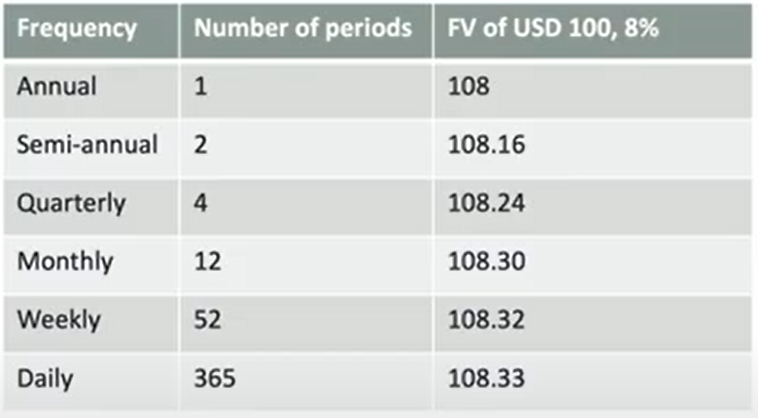
\includegraphics[width=0.7\textwidth]{1.png}
\label{loadings}
\end{figure}

\section{Непрерывное накопление}
Если процент начисляется непрерывно (ежедневно), текущая и будущая стоимость связаны этой формулой:
\begin{equation*}
    FV_N = PV_0\times e^{rT}
\end{equation*}
В этой модели:
\begin{itemize}
    \item $FV_N$ - будущая стоимость
    \item $PV_0$ - текущая стоимость
    \item $e$ - константа
    \item $T$ - время в годах
\end{itemize}
Можно преобразовать ставку с непрерывным накоплением к ставке с дискретным накоплением и наоборот:
\begin{align*}
    PV_0\times(1+\frac{r_m}{m})^{n\times m} &= PV_0\times e^{r_cT}
    \\
    r_c &= m\times ln(1+\frac{r_m}{m})
    \\
    r_m &= m\times (e^{r_c/m}-1)
\end{align*}

\section{Кривая спот-ставок (spot rate)}

Спот-ставка z(t) - доходность к погашению бескупонной облигации, которая будет погашена через t лет.

Кривая спот-ставок - это набор спот-ставок с разными датами погашения.
\begin{figure}[h]
\centering
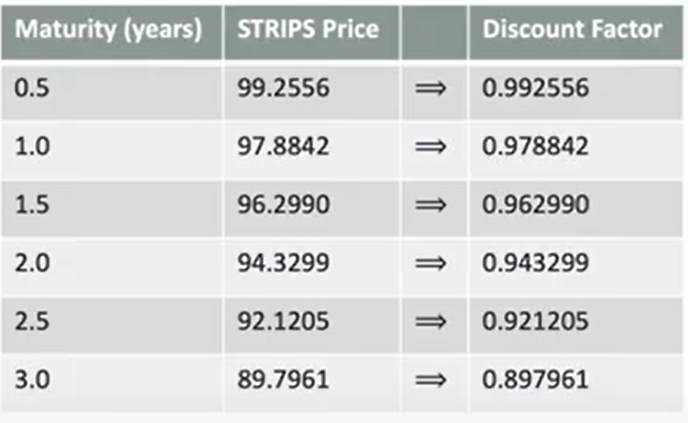
\includegraphics[width=0.7\textwidth]{2.png}
\caption{Пример: подсчет спот-ставок}
\label{loadings}
\end{figure}
Приняв $m=2$, используем формулу:
\begin{equation*}
    r = m[(\frac{FV_n}{PV_0})^\frac{1}{n\times m} - 1]
\end{equation*}
Получаем:
\begin{align*}
    t=0.5: 2\times [(\frac{100}{99.2556})^\frac{1}{0.5\times 2} - 1] &= 1.50\%
    \\
    t=1.0: 2\times [(\frac{100}{97.8842})^\frac{1}{1\times 2} - 1] &= 2.15\%
    \\
    t=1.5: 2\times [(\frac{100}{96.2990})^\frac{1}{1.5\times 2} - 1] &= 2.53\%
    \\
    t=2.0: 2\times [(\frac{100}{94.3299})^\frac{1}{2\times 2} - 1] &= 2.94\%
    \\
     t=2.5: 2\times [(\frac{100}{92.1205})^\frac{1}{2.5\times 2} - 1] &= 3.31\%
    \\
     t=3.0: 2\times [(\frac{100}{89.7961})^\frac{1}{3\times 2} - 1] &= 3.62\%
\end{align*}

\begin{figure}[h]
\centering
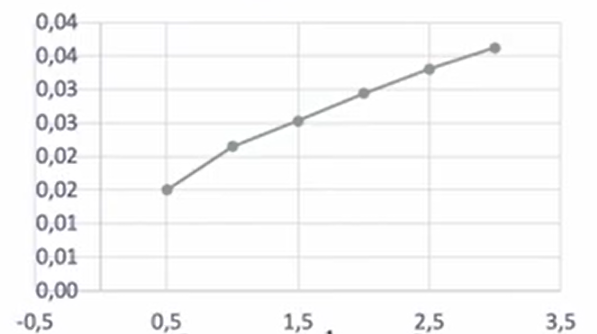
\includegraphics[width=0.7\textwidth]{3.png}
\label{loadings}
\end{figure}

\section{Форвардные ставки}

Форвардная ставка - это спот-ставка, которая, по мнению рынка, будет действовать через какое-то время. Эти ставки определяются текущими ожиданиями рынка, которые можно выразить через кривую спот-ставок.

\underline{Пример: } Найдем форвардную ставку. Пусть $z(1.0) = 2.15\%, z(1.5) = 2.53\%$

\begin{equation*}
    (1+\frac{0.0253}{2})^3 = (1+\frac{0.0215}{2})^2 \times (1+\frac{f(1.5)}{2})^1 \Rightarrow f(1.5) = 3.29\%
\end{equation*}

\begin{figure}[h]
\centering
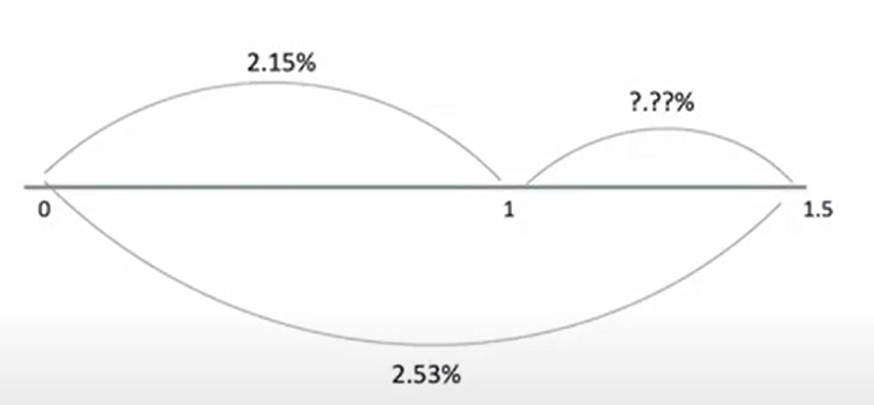
\includegraphics[width=0.7\textwidth]{4.png}
\label{loadings}
\end{figure}

\section{Номинальные ставки}
Номинальная ставка - это ставка периодического платежа, которая уравновешивает номинальную и текущую стоимость инструмента.
\begin{equation*}
    \frac{par rate}{m}(d(\frac{1}{m})+d(\frac{2}{m})+...+d(\frac{n\times m}{m}))+100d(\frac{n \times m}{m}) = 100
\end{equation*}
\underline{Пример:} Расчет номинальной ставки. Пусть $m=2, d(0.5) = 0.9968, d(1.0) = 0.9920, d(1.5) = 0.9848, d(2.0) = 0.9771$

\begin{equation*}
    \frac{par rate}{m}(0.9968+0.9920+0.9848+0.9771)+100\times 0.9771 = 100 \Rightarrow par rate = 1.16\%
\end{equation*}

\section{Сравнение спот-ставок, форвардных и номинальных ставок}

Попробуем выполнить прайсинг однолетней казначейской облигации, которая каждые полгода выплачивает купон по 4\%.

\begin{figure}[h]
\centering
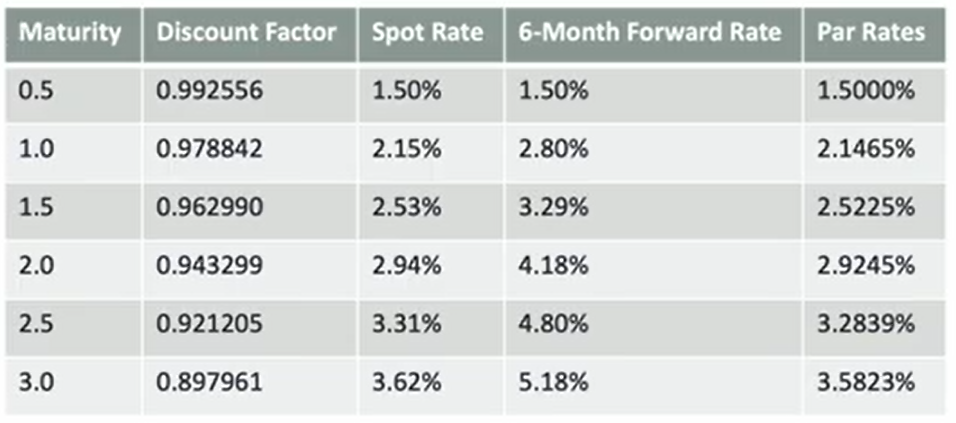
\includegraphics[width=0.7\textwidth]{5.png}
\label{loadings}
\end{figure}
\begin{itemize}

    \item Подсчет с помощью дисконт факторов:

    \begin{equation*}
        P = 2\times 0.992556+102\times 0.978842 = 101.83
    \end{equation*}

    \item Подсчет с помощью спот-ставок:

    \begin{equation*}
        P = \frac{2}{(1+\frac{0.0150}{2})^1} + \frac{102}{(1+\frac{0.0215}{2})^2} = 101.83
    \end{equation*}
    
    \item Подсчет с помощью форвардных ставок:

    \begin{equation*}
        P = \frac{2}{(1+\frac{0.0150}{2})^1} + \frac{102}{(1+\frac{0.0150}{2})^1\times(1+\frac{0.0280}{2})^1} = 101.83
    \end{equation*}

    \item Подсчет с помощью номинальных ставок:

    \begin{align*}
        P &= 0.978842\times 100 + \frac{0.04}{2}(0.992556 + 0.978842)\times 100 (1)
        \\
        100 &= 0.978842\times 100 + \frac{0.021465}{2}(0.992556+0.978842)\times 100 (2)
        \\
        (1)&-(2): P - 100 = \frac{0.04 - 0.021465}{2}(0.992556 + 0.978842)\times 100
        \\
        \Rightarrow P &= 101.83
    \end{align*}
\end{itemize}

\textbf{ЗАМЕЧАНИЕ:}

Каждая спот-ставка примерно равна среднему арифметическому форвардных ставок с такой же и более низкой датой погашения:
\begin{equation*}
    2.53\% \approx \frac{1.50\% + 2.80\% + 3.29\%}{3}
\end{equation*}

\textbf{ЗАМЕЧАНИЕ:}

Спотовые ставки растут с увеличением времени до погашения, значит, форвардные ставки должны быть больше, чем спот-ставки.

\textbf{ЗАМЕЧАНИЕ:}

Номинальные ставки немного ниже спот ставок.

\textbf{SUMMARY:}

Если структура ставок прямая (все ставки равны), то номинальные и форвардные ставки будут равны спотовым.

Если ставки растут по мере увеличения даты погашения, номинальная ставка для каждого срока всегда чуть ниже спотовой, а форвардная наоборот выше спотовой.

Если ставки снижаются по мере увеличения даты погашения, номинальная ставка для каждого срока всегда чуть выше спотовой, а форвардная будет ниже.

\section{Эффект от приближения к погашению}

По мере того, как облигация приближается к погашению, у нее остается все меньше невыплаченных платежей, а оставшиеся приближаются:

\begin{figure}[h]
\centering
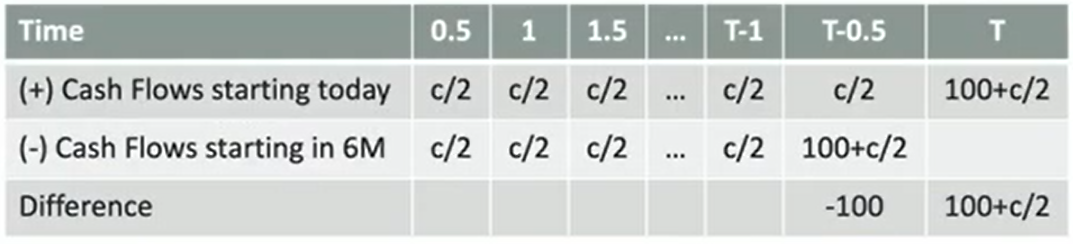
\includegraphics[width=0.7\textwidth]{6.png}
\label{loadings}
\end{figure}

Разница между стоимостью облигации сейчас и через 6 месяцев:
\begin{equation*}
    -100\times (1+f_T)+100+\frac{c}{2}
\end{equation*}
Поэтому эффект от приближения к погашению зависит от форвардной и купонной ставок.

Стоимости облигаций:
\begin{itemize}
    \item растут при приближении к погашению, если купонные ставки выше форвардных

    \item убывают при приближении к погашению, если купонные ставки ниже форвардных
\end{itemize}

\section{LIBOR и Overnight}

LIBOR (London Interbank Offered Rate) - ставка по которой банки в теории обмениваются между собой необеспеченными займами. Котируется в нескольких валютах и для разных сроков. Является преференсной ставкой для большого количества сделок.

Каждый день Британская Банковская Ассоциация (BBA) опрашивает набор самых крупных банков, по какой ставке те думают смогут получить фондирование у другого банка около 11AM (GMT). Далее отсекаются 25\% самых низких и 25\% самых высоких показателей, чтобы снизить уровень манипулирования ставкой банками. Оставшиеся показатели усредняются - это и есть LIBOR.

\textbf{LIBOR не идеален}
\begin{itemize}
    \item Это субъективная оценка банков.
    \item Банки могут пытаться манипулировать ставкой.
\end{itemize}

\textbf{Overnight rate}
\begin{itemize}
    \item По ней так же необеспеченно кредитуются банки в конце каждого дня.
    \item Банки с излишком средств относительно требуемых резервов могут одолжить деньги банкам с недостатком средств с помощью брокеров.
    \item В Амреике средняя ставка всех таких операций называется effective federal funds rate, то есть в отличие от LIBOR, ставка Overnight является продуктом реальных сделок.
\end{itemize}

\section{Свопы и своп-ставки}

Самый распространенный инструмент свопов процентных ставок - это plain vanilla interest rate swap (IRS).
\begin{itemize}
    \item Сторона 1 по этому контракту соглашается платить стороне 2 периодический фиксированный платеж, равный фиксированной ставке, умноженной на номинал сделки.

    \item Сторона 2 обязуется платить стороне 1 периодический плавающий платеж, который определяется как плавающая ставка, умноженная на номинал сделки.

    \item Все платежи в одной валюте.

    \item Обмен происходит только разницей в стоимостях.
\end{itemize}

\begin{figure}[h]
    \centering
    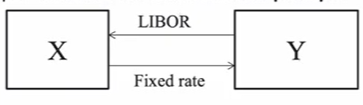
\includegraphics[width=0.7\textwidth]{9.png}
\end{figure}
Большинство IRS используют LIBOR в качестве референса для плавающей ставки.

\begin{figure}[h]
    \centering
    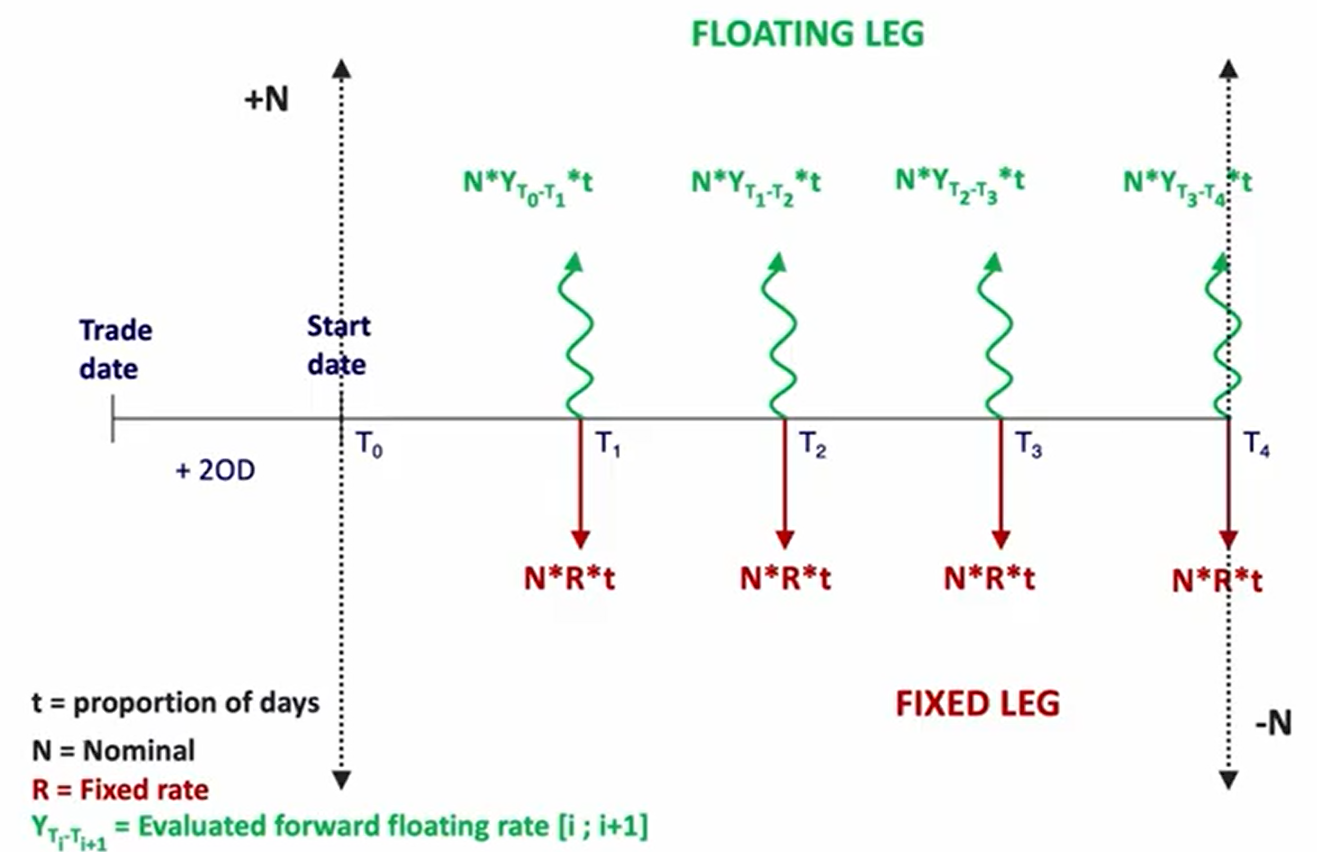
\includegraphics[width=0.7\textwidth]{10.png}
\end{figure}

\section{Получение дисконт факторов из IRS}

Можно представить fixed leg и floating leg в виде облигаций. Единственная разница - нет обмена номиналом.

Тот, кто выплачивает фиксированную ставку и получает плавающую, "купил" облигацию с плавающей ставкой. Тот, кто получает фиксированную ставку и выплачивает плавающую, "покупает" облигацию с фиксированной ставкой.

\Rightarrow

Своповые ставки = купонные платежи

Номинал свопа = номинал облигации

Фиксированная ставка - аналог номинальной ставки облигации

\underline{Пример: } Расчет дисконт ставок из ставок свопов.
\begin{figure}[h]
    \centering
    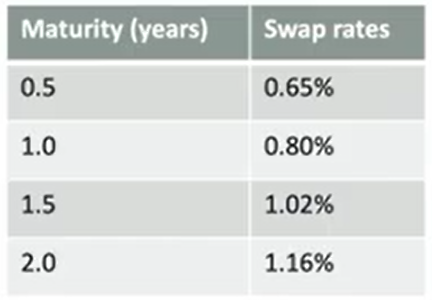
\includegraphics[width=0.7\textwidth]{11.png}
\end{figure}
Номинал = 100

Решение: считаем фиксированную ставку свопа как номинальную ставку облигации

\begin{align*}
    100 &= (100 + \frac{0.65}{2})\times d(0.5) \Rightarrow d(0.5) = 0.9968
    \\
    100 &= (100 + \frac{0.8}{2})\times d(1)+(\frac{0.8}{2})\times d(0.5) \Rightarrow d(1) = 0.9920
    \\
    d(0.5) &= 0.9968
    \\
    d(1.0) &= 0.9920
    \\
    d(1.5) &= 0.9848
    \\
    d(2.0) &= 0.9771
\end{align*}

\section{Overnight index swaps (OIS)}

OIS в качестве референсного значения, вместо LIBOR, использует геометрическое среднее Overnight ставок.

Ставки по фиксированной ноге в OIS называются OIS rates.



\section{Процентные кривые и их изменения}

\begin{figure}[h]
    \centering
    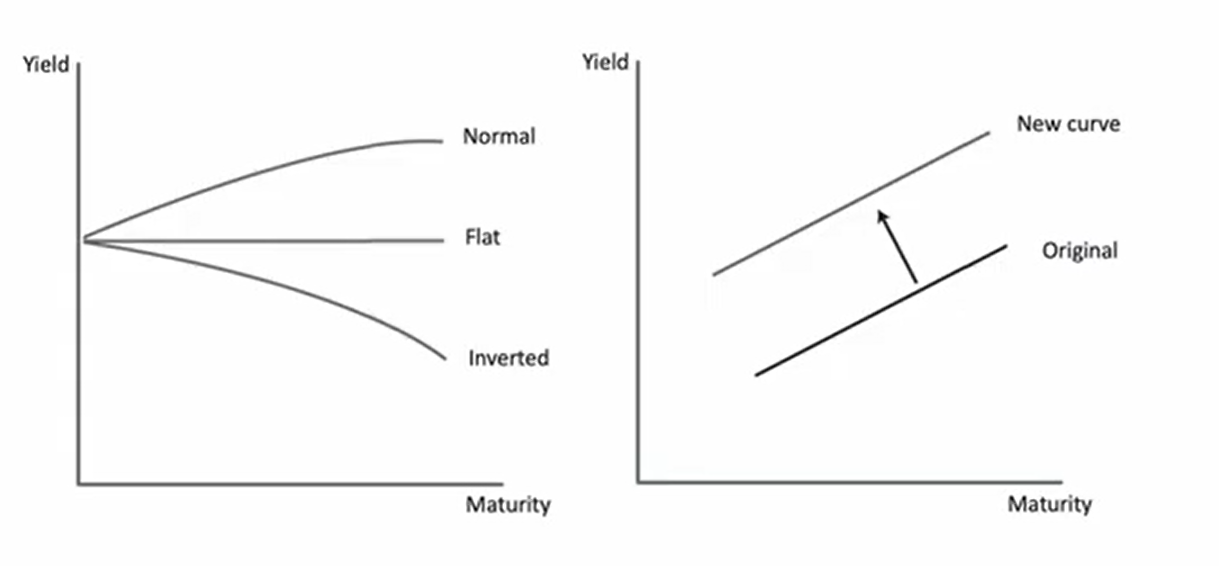
\includegraphics[width=0.7\textwidth]{7.png}
\end{figure}

\begin{figure}[h]
    \centering
    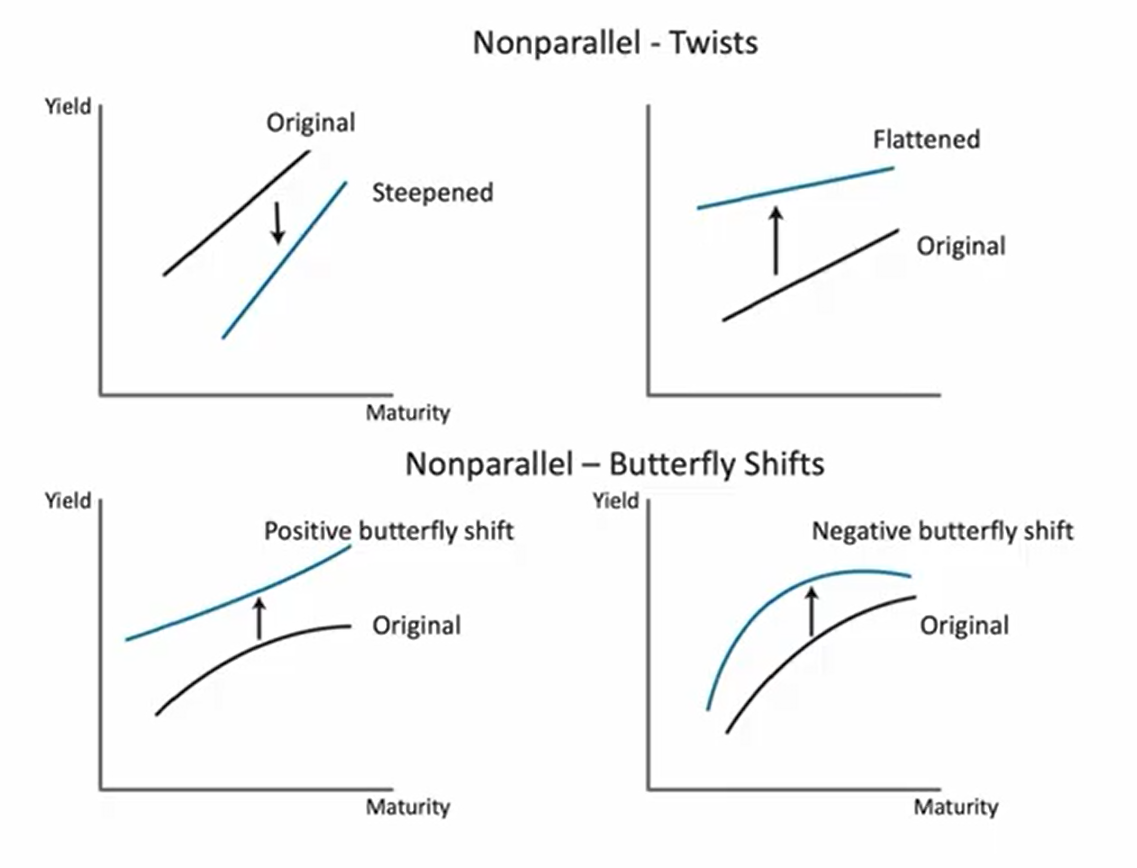
\includegraphics[width=0.7\textwidth]{8.png}
\end{figure}

\end{document}




